%% rm report.pdf ; pdflatex -halt-on-error report.tex  && evince report.pdf
%% latex x.tex ; evince x.dvi

\documentclass[10pt,a4paper]{article}
% \documentclass[12pt]{report}
\usepackage{amsmath}

% gives us \url 
\usepackage{hyperref}

% indent the first para after a new section
%\usepackage{indentfirst}

% for png
\usepackage{graphicx}
\graphicspath{ {images/} }



% for figure captioning
%\usepackage[capposition=top]{floatrow}
%\usepackage{caption}
\usepackage{caption}

% to control positioning
\usepackage{float}

% missing - \usepackage{sectsty}


% control section fonts - it does work
\usepackage{sectsty}
\subsectionfont{\fontsize{10}{10}\selectfont}

% italic environment
\newenvironment{italicquotes}
{\begin{quote}\itshape}
{\end{quote}}

% bullet point lists
\let\Item\item
\newcommand\SpecialItem{\renewcommand\item[1][]{\Item[\textbullet~\bfseries##1]}}
\renewcommand\enddescription{\endlist\global\let\item\Item}

\title{Investigation into Control Vocabulary Publishing Services}
\date{}
\begin{document}
\SpecialItem

  \maketitle
    \begin{flushleft}


%  \setlength{\parindent}{5ex}

% 
% \section{High level requirements}
%   \item[Text] more text
%     and below
%   \item[and some] more text
%   \item[] empty
% \begin{italicquotes} hopefully italic  
%   and more italic
%   \end{italicquotes} 
% \url{http://www.uni.edu/~myname/best-website-ever.html}
% 

% need to be consisistent.


\section{
	Summary
}

\item[] IMOS/EMII should avoid pursuing our own ad-hoc solution and instead 
focus on integrating other provider's services and products to match needs due 
to limited development resources
\item[] LDP and SISSVoc should be considered complementary solutions rather than alternatives
\item[] It is not evident that centralised registration management such as 
that provided by LDP necessarily matches IMOS/EMII organisational publishing 
requirements. Even LDP authors acknowledge that their project is contrary to the 
non-federated nature of RDF publishing - while SISSVoc deployments appear to work
well independently  

\item[] Support for more sophisticated vocabulary authoring and development 
activity probably does not exist yet in the form of a web-based solution. For 
example, to support inferencing and consistency checking of OWL vocabularies already 
found in dedicated third-party vocabulary applications, or to verify the 
reciprocal relationship of broader/narrower SKOS terms.
\item[] An investment has already been made in the development of a controlled vocabulary 
database. This includes supporting the appending of Geoserver parameter and 
unit information at WFS download and 
as a source of SKOS vocabulary for Geonetwork/Portal 123 for faceted search. 
Abandoning this effort would require the establishment of new work-flows as well as infrastructure
changes
\item[] LDP is currently unfunded, lacking project oversight, technical 
support, points of contact or active discussion forums. It clearly presents an infeasible technical-risk 
unless there is a consensus from multiple external groups on new funding and 
feature development 


\clearpage

% multiple SISSVOC publishers have emerged and co-operate well together 

% have a section on background

\section{
  Tasks undertaken
}

%  
  The following tasks were completed:  

    \item[] A local instance of SISSVoc using preconfigured external SPARQL
  endpoints for various service providers was run-up under a tomcat webserver and
  demonstrated during Iteration review.  \footnote{ \url {
  http://github.com/jyucsiro/SISSVoc-runner }  } 

    \item[] It was very difficult to glean an understanding of the
  functionality of LDP by reading source-code and internal development
  literature. Therefore a version of UKGovLD was also run-up on a private Nectar
  VM allocation. This followed prior unsuccessful attempts to provision a vagrant
  example of UKGovLD.  \footnote{ \url {
  https://github.com/UKGovLD/registry-deploy-poc } and \url {
  http://ukgovld-registry.s3.amazonaws.com/distribution/ukl-registry-0.0.1-SNAPSHOT-dist.tar.gz
  } }
  %
    Attempting to generate a dummy configuration for LDP and login with
  administrative privileges was frustrated, due to an apparent bug in open-id redirection.
  However it was possible to explore and navigate the main menu-system of the
  application.
  %
    The discussion of LDP features is therefore more limited.

    \item[] Preliminary scripts to extract and encode the contents of the IMOS
  controlled vocabulary database as SKOS were written to guage the difficulty to
  perform the required mapping. These were further modified to be suitable to
  input into Geonetwork for current development to support platform / parameter
  based faceted search. Such export feature would probably also be necessary for
  upload to a publishing provider eg. ANDS or purl.org. 

    \item[] Attempted to register with ANDS and obtain an account to establish a
  test registry of published vocabulary terms. There were some technical issues,
  requiring help from ANDS technical support which were unresolved.
      
    \item[] SISSVoc and LDP was assesed against the \textit{High Level Functional
  Requirements For Vocabulary and Term Publishing} previously prepared by Project
  Officers.
    

\clearpage


\section { 
	High Level Functional Requirements For Vocabulary and Term Publishing
}

% OK
% 1 
  \subsection{
   Main function is to provide a resolvable endpoint for a vocabulary and its
  included terms (and details) using persistent identifiers.* 
  }

  \item For each term in the vocabulary persistent identifiers {URI} should
  be de-referenceable to the RDF item description. 

  \item SISSVoc as a standalone application has no inherent support for managing persistent
  identifiers. The main SISSVoc paper describes a deployment \footnote{ See Figure 3,
  SISSVoc: A Linked Data API for SKOS vocabularies.

  \url{http://www.semantic-web-journal.net/system/files/swj658.pdf} }, using a
  Persistent Identifier Service to map persistent URI resources to SISSVoc
  webservice urls, but fails to give futher details on the implementation or
  whether an external provider was chosen. 

  \item ANDS controlled vocabulary services builds upon SISSVoc, although it appears
  their persistent identifier service may be a more general organisational capability. According to
  documentation ANDS has, 

  \begin{italicquotes} [...] a simple HTTP-based interface, [which] ensures that
  identifier services can be integrated easily into existing data management
  workflows.  \end{italicquotes}
  Futhermore, ANDS does undertake to persist the infrastructure required for
  keeping its identifiers online. Ideally this service would be integrated
  with other SISSVoc vocabulary management functionality, although this was not tested.

  \item[]Another alternative, would be to use a service such as \url{purl.org} which is a free provider 
  of Persistent Uniform Resource Locators, that includes high-level adminstrative functionality including 
  Users, Groups, Domains, Help etc.  \footnote{ 
  The most prominent instances of such schemes are PURLexternal link, which has been used
  by the National Library of Australia, and ARKexternal link, at the California
  Digital Library.  }. 

  \item[]It would probably also be a simple step to publish identifiers under an
  AODN or EMII DNS controlled url. In this context, Seegrid appear to have developed their own
  PID service used in conjunction with their own SISSVoc deployment  \footnote{
  https://www.seegrid.csiro.au/wiki/Siss/PIDService}  
  
  \item[]LDP is a resource registry management system, however it is unknown 
  if this includes direct support for persisent identifiers.
    \footnote{ See 
    https://github.com/UKGovLD/ukl-registry-poc/wiki/Principles-and-concepts
  }


% LDP -   The API should, where reasonable, follow REST principles. Specifically that
% any resource in the system should be identified by a URI and be manipulable by
% standard HTTP verbs (GET, PUT, DELETE, PATCH).
% 

% also supports versioning and management of PID could
%% ok, we got this restful stuff confused. GET,POST,DELETE,UPDATE... etc.
%% are html commANDS.

%   \# SISSVoc Deployment complemented by PID service
%   PURL. SISSVoc used a per
%   \url{https://www.seegrid.csiro.au/wiki/Siss/PIDService} 
% 
%   
%   SISSVoc - locally or externally hosted (ANDS) supports using persistent
%   identifiers.  Article tals branding. 4 things - expected.  Talk about RDF.
% 
%   SISSVoc is built upon RDF, and is a restful publishing api. 
%%   The DNS resolvable component of the uri, it is expected that ANDS will maintain
% 
%   ANDS and IMOS has extensive experience in managing in chef the DNS component of
%   names. Alternatively ANDS
% 


%% OK
% 2
\subsection{Resolvable content should be structured (or at least be able to be queried)
  using an RDF/SKOS encoding model. Content may however be adorned by other
  languages/metadata models (e.g. RDFS, OWL, Dublin Core).* }

  \item SISSVoc provides a linked data API for publishing SKOS vocabularies. SKOS
  is a standard vocabulary for thesarui, classifications, taxonomies and
controlled vocabularies using RDF.

   \item  The SISSVoc web-service API supports URI patterns that are aligned with the SKOS
  vocabulary model. This includes access patterns for SKOS Concept,
  ConceptScheme and Collection. Further URI patterns are provided to discover
  broader and narrower terms in transitive and non-transitive forms and according
  to text based labels. 

     \item SKOS can be decorated with other RDF based content and persisted to
  any underlying relational or triple store independently of SISSVoc
  functionality. However, SISSVoc provides no direct support URI patterns for the
  search and discovery of such content. As an alternative, a SPARQL interface
  does provide a query/search mechanism for non-SKOS content such as DC, RDFS or
  OWL classes. A local-instance of SISSVoc could be modified to use this SPARQL
  with support in the GUI if such functionality was deemed important. 

  \item It is believed that LDP has no specific API support for SKOS resources.

%    According to Cox, SKOS lacks the expresitivity of languages such as OWL.
%   However common metadata standards like Dublin Core are supported.
%     It is anticipated that SKOS can be decorated with any data/metadata that can
%   be encoded in RDF triples.
% 
%   Additionally the SKOS Extensions RDF Vocabulary are a set of terms extending
%   the SKOS Core vocabulary to support some common features of knowledge
%   organisation systems, especially thesauri. (link) The extensions would appear
%   to be designed to cover common needs for representing authoring and publishing.
% 
%   Resolvable content - can be extracted SKOS Concepts from the already developed
%   relational vocab database demonstrates another approach which can then be
%   ingested to a RDF persistence. An example script has been created to demonstate
%   the feasibility of this approach. Alternately a SPARQL interface to RDF could
%   be used over the , to form RDF/SKOS content.
% 

% OK
% 3 
  \subsection{
  It should be possible to access vocabularies and their terms via an 
  (administratively) customisable Web-client interface and service interfaces.* } 

   \item  SISSVoc provides a capable Web-client interface for read-only access
  vocabularies and their terms.

   \item  In contrast to search, naviation and discovery, SISSVoc as a standalone
  application has no direct support for the creation and update of vocabulary
  terms. This is inherent to SISSVoc design, as a lightweight web-api implemented
  over a read-only based SPARQL endpoint/interface.  

  %   the SISSVoc client interface supports customisation, image branding which
  %   can be achieved via changes to css and js configuration.  Examples are
  %   given in the source code.  \footnote {
  %   https://github.com/jyucsiro/SISSVoc-runner/tree/master/SISSVoc/resources }
  %    
 \item    According to the ANDS handbook, ANDS provides web-based GUI support for
  editing SKOS but only at file level.  \footnote { See 3.4.3, Editing
  Vocabularies \url{ http://www.ANDS.org.au/support/vocab-help-guide.pdf } } Some 
  support for web-based versioning and author management at the file level
  is also available. While permissions to make change are tied to authority 
  roles.  \footnote { There is a need to consider whether file level versioning and
  management is sufficiently fine-grained. Also how should this interact with
  existing registry management already used in IMOS \texttt{control\_vocab\_db}.
  }
    
  % this doesn't quite belong, 
 \item    For complex vocabulary authoring needs, SISSVoc authors suggest using an
  external vocabulary editor to maintain content that can also ensure that
  consistency of relationships between resources is maintained (eg. for OWL). 

    \begin{italicquotes} Vocabulary content may be maintained using RDF editors
  (such as Protégé 4 or TopBraid Composer 5 ), which ensure consistency of
  relationships between resources is maintained, and then generate RDF documents
  to transfer vocabulary content from the maintenance to publication envi-
  ronment, as outlined above. If a web-based vocabu- lary maintenance environment
  is required, then tools like TopQuadrant’s Enterprise Vocabulary Net 6 , and
  the PoolParty Thesaurus Server 7 are available.  \end{italicquotes} 

    \footnote { 3.2. SISSVoc HTTP operations and REST behaviour discussed,
  \url{http://www.semantic-web-journal.net/system/files/swj658.pdf} }


% OK
% 4
\subsection{ 
  Most users require read only access to content.* 
}
  \item SISSVoc provides an easy-to-use Web-client interface for read-only access to 
  vocabularies and their terms.  As already noted SISSVoc has a read-only application design.
 
  \item LDP provides a Web-client for fine grained registry management of term
resources. But this is a believed to be a general capability lacking SKOS specific support.


% OK
% 5
\subsection{ 
  There should ideally be a service interface that is REST-based* and a 
  SPARQL service end-point.
}

     \item SISSVoc is designed with a HTTP-based interface aligned with
  REST-based web services. The URI patterns facilitate SKOS discovery and access.
  However, as the authors of the system note, SISSVoc is not a full RESTful API, as 
  it does not support HTTP operations for update and deletion of resources.
      
    \item  LDP is designed with a view to RESTFUL management of registry
  resources.  \footnote { https://github.com/UKGovLD/ukl-registry-poc/wiki/Api }
  It should be noted that references to SKOS in the discussion of the LDP api
  apply to registrars, not SKOS content maintained by particular registrants.  

      \item SPARQL (Simple Protocol and RDF Query Language) is an RDF query
  language able to preserve, retrieve and manipulate data in RDF format and is a
  W3c standard.  SPARQL abstracts the encoding model (XML, … etc), and
  persistence layer and is adapted to the non-relational / graph structure of
  RDF.

   \item   The SISSVoc RESTFUL URI patterns correspond quite closely with
  specific SPARQL queries which perform the substantial computation. SISSVoc thus relies
  on a SPARQL endpoint as the mechanism to access RDF providing a strong
  separation of concerns. It would be feasible to map the already developed IMOS
  \texttt{control\_vocab\_db} to expose a SPARQL interface using a tool such as
  r2rml \footnote{ \url{ http://www.w3.org/TR/r2rml/ } }. This has already been
  achieved in one controlled vocabulary instance \footnote{ \url{ http://www.seb-source.org/ } }. 
  The SPARQL interface would thus provide the endpoint for SISSVoc and replace the 
  need to manage an additional persistence layer.

  \item It is expected that an external SISSVoc provider such as ANDS would be 
  unlikely to expose such a low-level query capability.
   

% OK
% 6
\subsection{ The publishing and retrieval service should offer and receive
re-direction(s) so that vocabularies or terms hosted on different domains (under
differing content authorities) can still be accessed via the service (if
desired). * }

  {
  \item SISSVoc supports seamless and consistent GUI based navigation between differing
  SISSVoc instances hosted on different domains.
  %
  \item Alternatively, normal URI de-referencing allows navigation to non-SISSVoc
  vocabulary implementations and their terms (eg. BODC/NERC).
  %
  \item Interestingly, due to the nature of the decoupled end-point design, SISSVoc 
  can be configured to use multiple SPARQL endpoint providers. This unifies access
  to different vocabulary providers that expose SPARQL from the same SISSVoc instance. 

  % H=HERE
  \begin{figure}[H]
  \centering
  \caption{SISSVoc host demonstrating access to multiple SISSVoc domains from the same instance}
  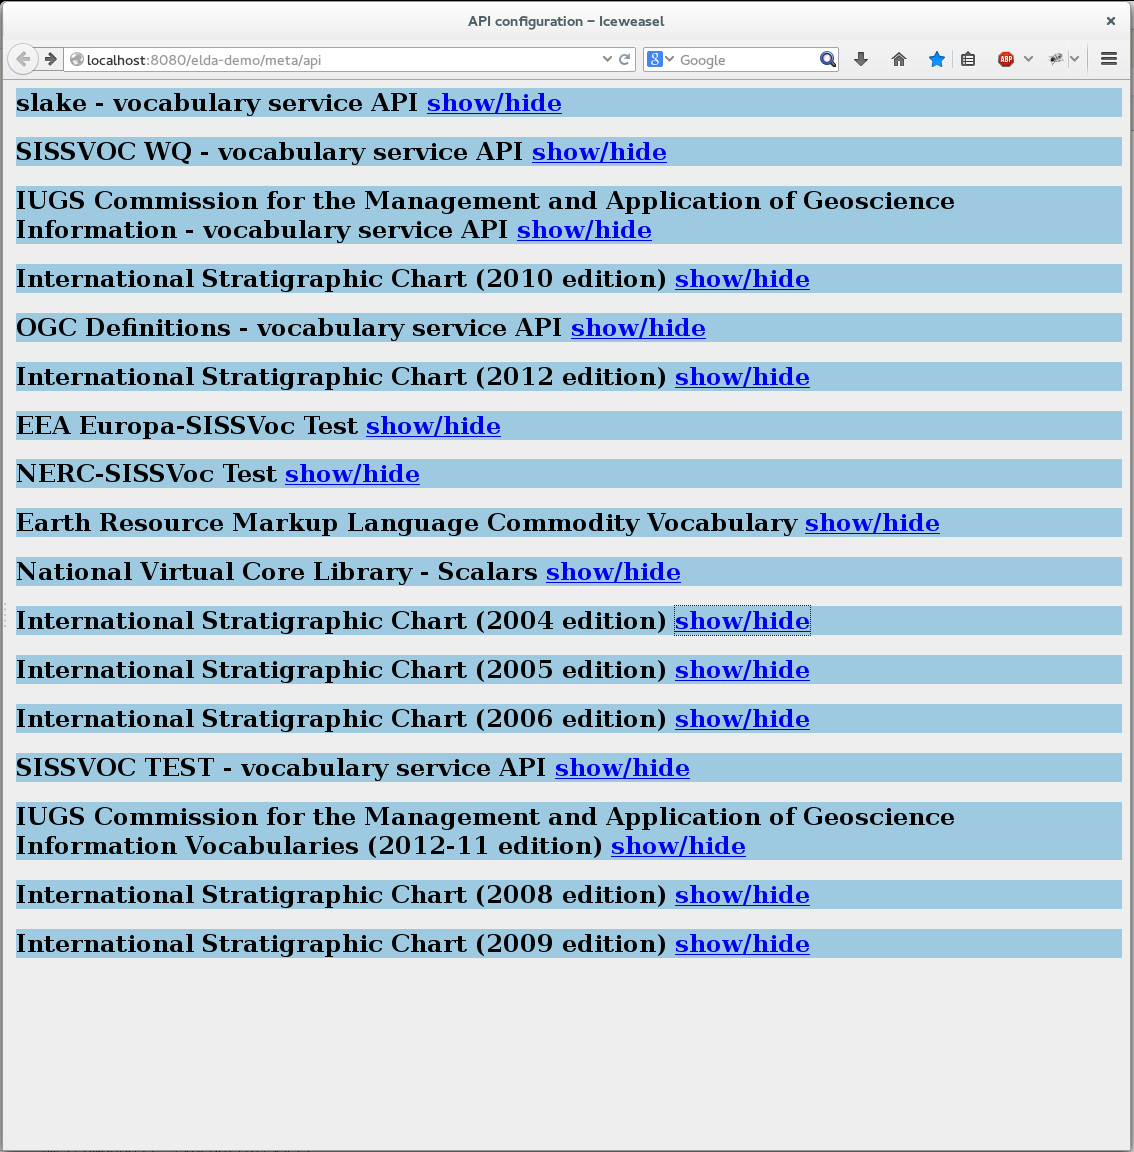
\includegraphics[width=12cm]{multipleendpoints}  
  \label{fig:test}
  \end{figure}

  LDP GUI navigation capabilities are unknown, but assumed to be limited to 
  registry management.
  }
  %
%
% CRAP  - Maybe OK
%7
\subsection{ The Web-client should support some basic ‘canned’ querying (e.g.
free text search against concept, collection and scheme ‘labels’; traversing a
named vocabulary via hypertext links to explore included terms, their details
and any matches or mappings to other published vocabularies). * }
%
  \item SISSVoc supports free-text searching against concept labels. It can list
  concept, collection and concept schemes. SISSVoc can also traverse links 
  for associated broader and narrower terms. 

  \begin{figure}[H]
  \centering
  \caption{SISSVoc Gui Concept search and results}
  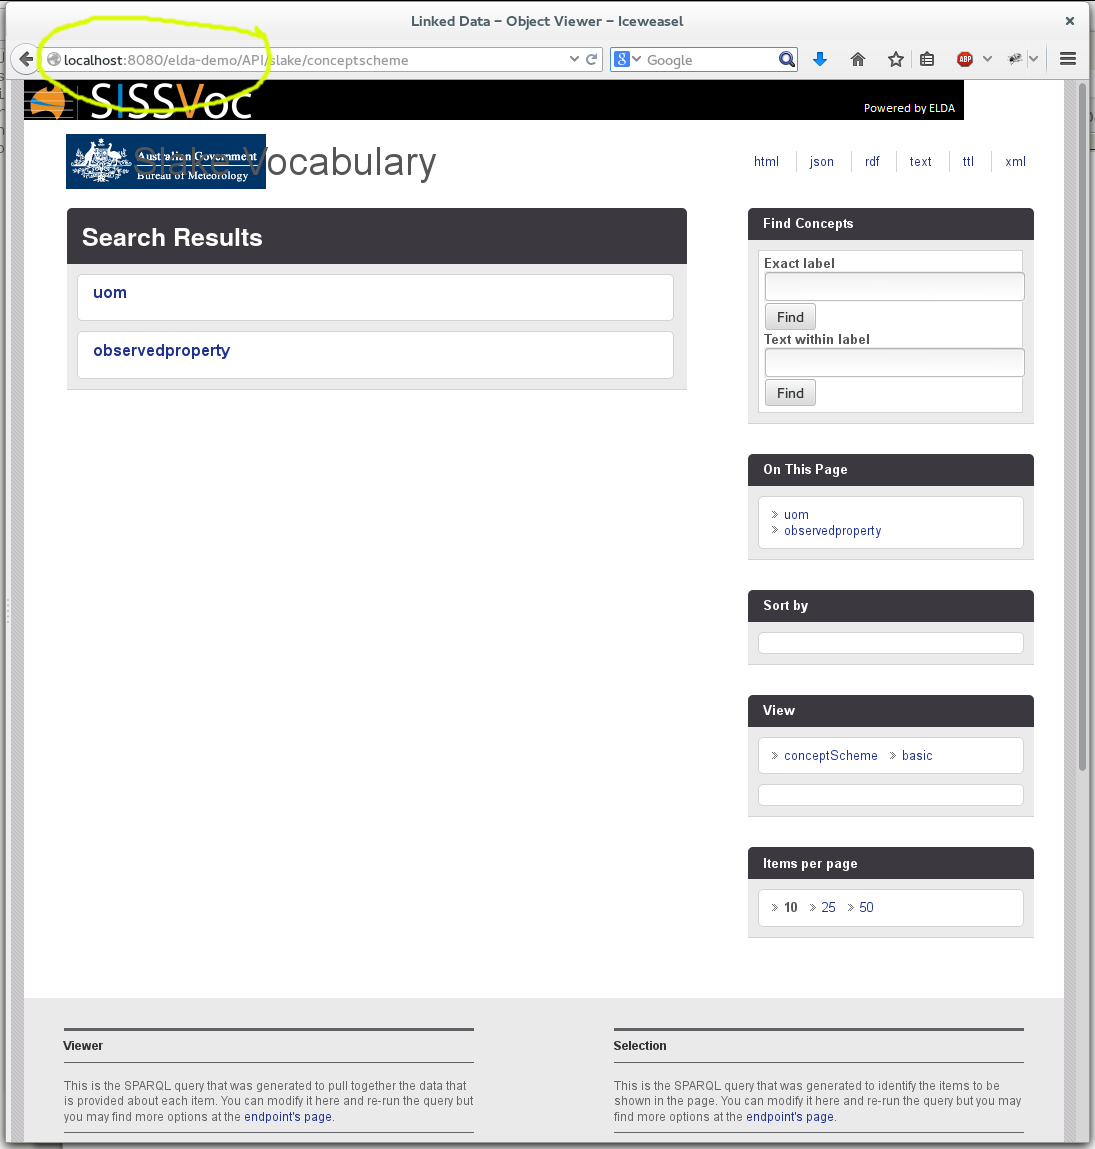
\includegraphics[width=12cm]{sissvoc}  
  \label{fig:test}
  \end{figure}



  % SISSVoc - yes (local instance). configurable ttl - examples available.
  % SISSVoc configuration is in RDF using TTL encoding. Lots of examples are given. 
  % Need to assess - concept, collection, scheme each one individually.
  % ANDS SISSVoc has also developed a vocabulary tree style widget
  % https://researchdata.ANDS.org.au/developers/documentation/widgets/vocab_widget
  % 

LDP capabilities for registrar searching are unknown.


% OK
% as an alternative protoge with a dedicated SKOS and OWL plugins. 
% 8
\subsection{ The Web-Client should be able to display in a user-friendly way
(e.g. using tables or forms) vocabulary and term details (e.g. scheme,
collection and concept labels; alt labels, its type, description, membership,
relations [including some Dublin core relations such as ‘publisher’ and ‘owner’
and revision info]). * }

\item The SISSVoc Web-Client supports user-friendly presentation of SKOS term details
including preferred label, definition, broader, and membership relations. Also
other metatadata terms such as DC. 

\item It appears that the simple html table layout supports showing all associated RDF
properties if they are literals or RDFs:label types rather than URIs that
need to be de-referenced.

\begin{figure}[H]
\centering
\caption{SISSVoc Gui SKOS Resource }
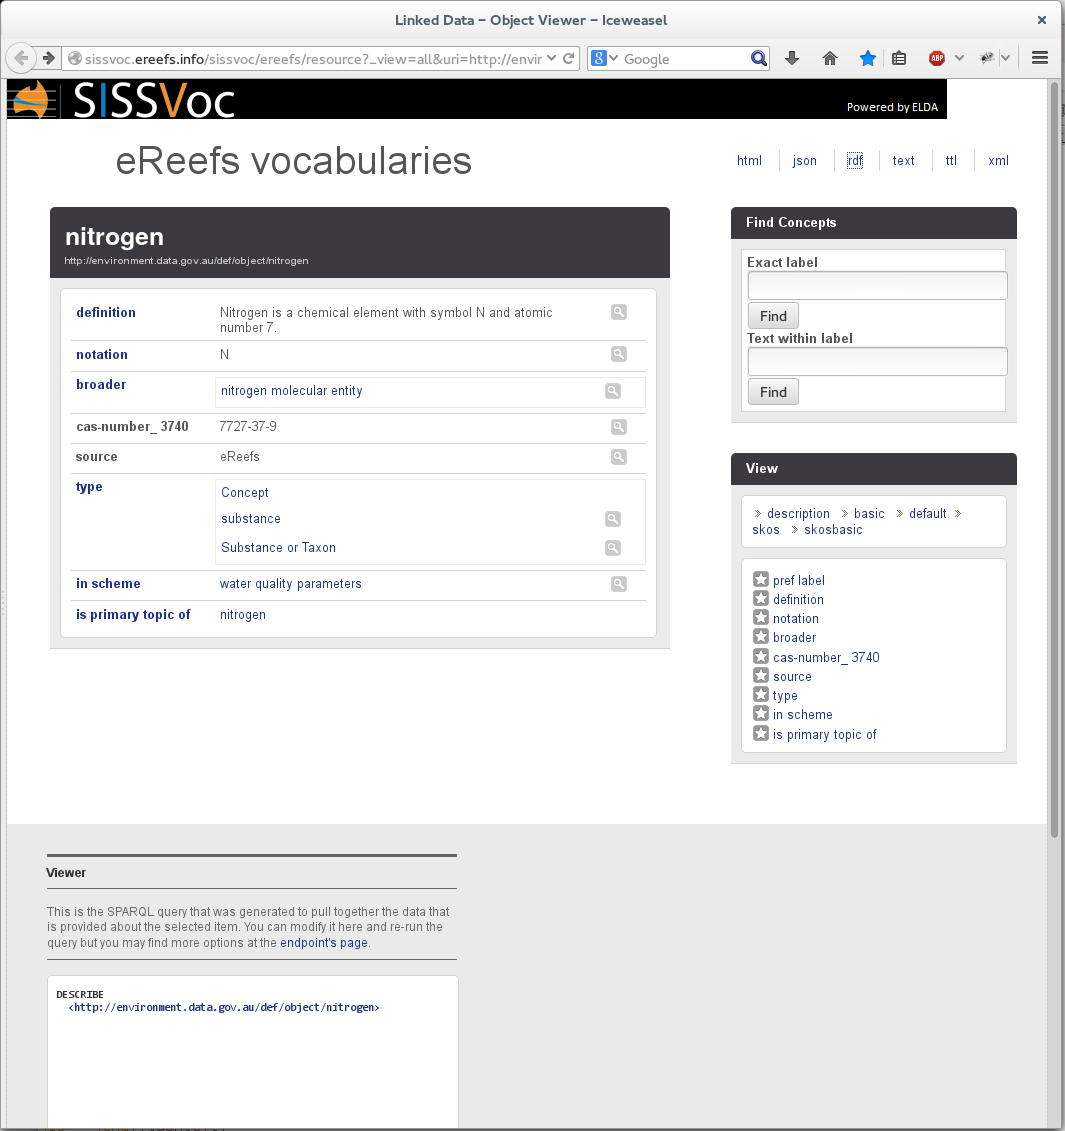
\includegraphics[width=12cm]{nitrogen}  
\label{fig:test}
\end{figure}


%%%%%%%%%%%%%%

% OK although brief.
%9 
\subsection{ The Web-Client should be able to display categorized
(classified) lists of discoverable content (e.g. all vocabs by provided by
owner X; all terms in vocab Y) }

%owner - meaning - repo management.  classification - ?? must learn

  \item[] SISSVoc as a stand-alone application has no notion of term ownership semantics. There is
  a set of extensions for SKOS that appear to be designed to support management such as 
  assigning author properties. 
  \footnote  { \url { http://www.w3.org/TR/skos-reference/skos-xl.html } }    
  % importance of SKOS_XL Presumably  

  \item[] ANDS may have support since it combines some registry management with SISSVoc. 

  \item LDP unknown, although conceivable since consistent with registry management function.


% OK
% 10 
\subsection{ The Web-Client should offer different formats in which to
download vocabularies or their terms (e.g. RDF*, text*, json, html*) }

  \item SISSVoc supports download in human and machine readable form including html, 
  json, RDF, text, ttl and xml. However, the web-api has no support for downloading 
  partial or complete SKOS vocabularies except via a manually crafted SPARQL request.

  \item LDPs encoding support is unknown.

% ALMOST OK
% 11 
\subsection{ The Web-Client should offer some statistics for users on the
type and volume of content available (e.g., number of vocabularies that can be
accessed and the number of terms in each vocabulary).  }
 

  \item SISSVoc has no inherent support for compiling vocabulary content statistics.

  \item However, using a SPARQL interface it ought to be trivial to construct queries to identify
  for example the number of SKOS concepts, schemes or collections available with varying
  search constraints applied. 

% ALMOST OK
% 12
\subsection{ The publishing and retrieval service should be capable of
being configured to dynamically read one or more repository sources to access
content that needs to be published. * }

  \item As has been described, a stand-alone SISSVoc test-runner can be configured to
  read from multiple end-point data sources. Although the front-end GUI support is not
  very polished and uses styling inconsistent with the rest of the
  application.


% OK
% 13
\subsection{ 
Response times for retrieving queried content should be ‘user-tolerable’. *
}

\item During basic user-interface testing, both the local and remote ANDS
options assume appear to be responsive.

% It's expected that most of the speed will be backend / perssistence. 


% OK 
% 14
\subsection{ System should provide an administrative console/configuration
files to enable simple maintenance and administration (e.g., small changes to
Web-client interface displays and supported queries; to detect and fix broken
links in client-based hypertext; detecting missing details in retrieved content
– indicating content needs moderating/validating; provide basic statistics on
service usage).
}

  \item It's believed that neither SISSVoc or LDP offer any administrative control over configuration. 

  \item A locally deployed SISSVoc would permit the normal configuration possibilities that comes with 
  controlling the source code - such as css, ttl and javascript and xslt changes. Extended examples are
  provided for different branding options.

  \item For a local deployment, usage statistics could be compiled using awstats, in the same fashion as other 
  IMOS web-applications. 



\subsection{ 
There should be ‘meaningful’ error messaging provided in response to
service calls that cannot be satisfied (or which have been framed incorrectly).
* }

  \item SISSVoc and LDP appear to support basic error handling.




  \end{flushleft}

\end{document}

